\chapter{Testing and Evaluation}

In this chapter we present how the testing and evaluation of the proxy was
performed and present the results we obtained.  The goal is to measure any
possible improvements (or deterioration) of the performance of Web services when
the proxy developed as a part of this thesis is being used. Since the proxy was
developed as a prototype for military usage, we wanted to use test scenarios
that resembles actual military and civilian usage. For the purpose of testing,
we therefor originally developed two set of applications, one W3C Web service
and one RESTful Web service. These applications were then put to test in
networks with different characteristics. During testing, we discovered that some
of the protocols were very sensitive to the size of the messages being sent. We
therefor also developed a complementary test service which allowed us to test
sending messages of different sizes.

We'll get started by discussing the test and evaluation tools used, before we
introduce the different test applications, test cases and the different types
of networks used for testing. Then we present the test results for each of the
three aspects of DIL, \textit{disconnected, intermittent} and
\textit{limited.} The aspects were tested separately. We started with the
disconnected and intermittent tests, where we investigated the behaviour when
connection was lost. For the limited tests, we saw how different types of
networks influenced the performance of Web services. The base case was to
test without any intentional limitations to the network and without the actual
usage of the proxy. Then we introduced usage of the proxy and evaluated it in
different types of limited networks.

Furthermore we performed tests with two setups, first with machine-to-machine
over an Ethernet cable, then we supplemented with testing over actual military
communication equipment. The usage of actual military equipment allowed us to
get as realistic results as possible.

\section{Types of DIL networks}

Military communication can occur over a wide range of different technologies and
environments. These include \glsentryfull{satcom}, \glsentryfull{los},
\glsentryfull{cnr} and WiFi. WiFi is divided into two types to illustrate both
with good connection and one with less. Some communication technology, such as
Satellite communication, is characterized by long communication delay while
others may be by their low data rate. An overview of military communication
technologies can be seen in \cref{figure-networks-overview}.

\begin{figure}[h]
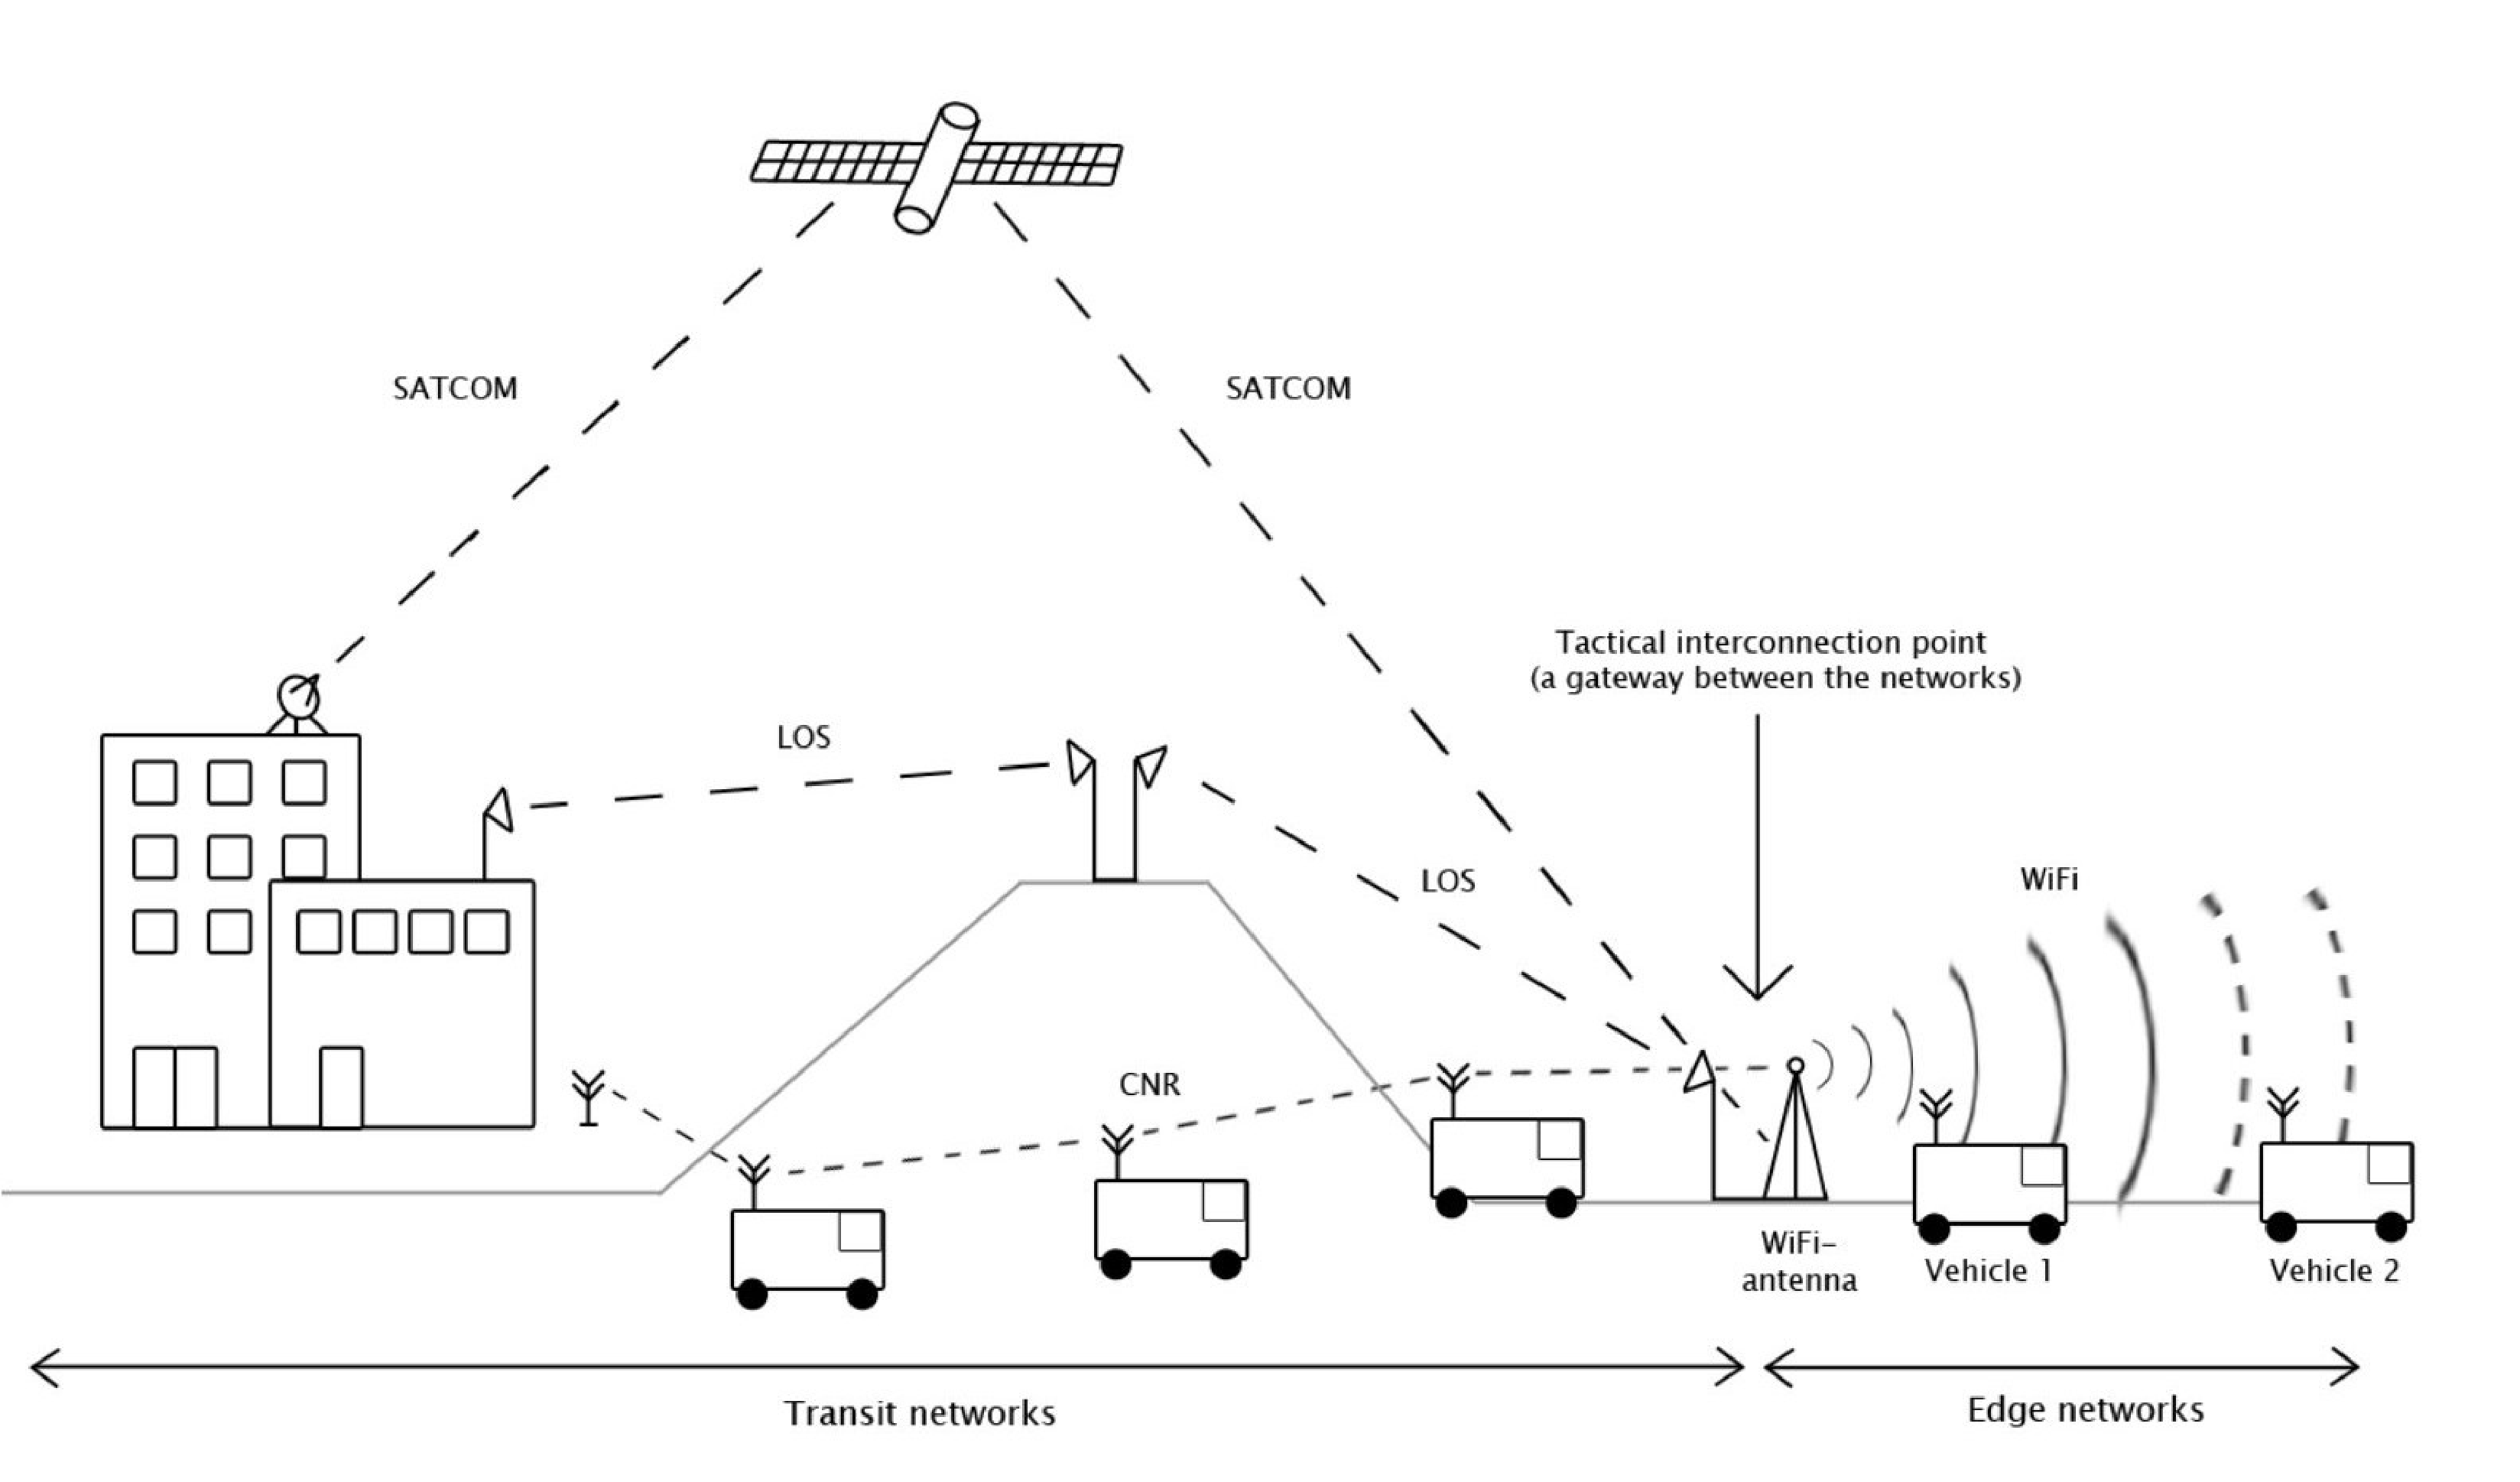
\includegraphics[scale=0.25]{images/networks_overview.pdf}
\caption{Overview of tested networks}
\label{figure-networks-overview}
\end{figure}

An infinite number of possible network combinations exists, so we have in this
thesis chosen to focus on five different network types identified by the task
group IST-118 for DIL-testing. We also investigated \gls{lte}, commonly known as
4G, a network technology which has become in widespread use in the latest years.
The reason for including LTE in addition to the ones from IST-118, is that the
Norwegian Defense is looking into the possibility of using LTE. Thus making it
interesting for us to investigate the performance under this type of network as
well. However, we eventually found out that LTE has gotten so fast and reliable,
that it is not really relevant from a DIL perspective. We therefor instead
looked into \gls{edge}, which is used as a fall back in geographical areas where
\gls{lte} and 3G is not available. The different networks and their properties
are summarized in \cref{table-network-types}.

\begin{table}[h]
\begin{tabular}{| l | l | l | l | l |}
\hline
  \textbf{Network} & \textbf{Data Rate} & \textbf{Delay} & \textbf{PER} \\ \hline
  Satellite Communication & 250 kbps & 550 ms & 0 \% \\ \hline
  Line of Sight & 2 mbps & 5 ms & 0 \% \\ \hline
  WiFi 1 & 2 mbps & 100 ms & 1 \% \\ \hline
  WiFi 2 & 2 mbps & 100 ms & 20 \% \\ \hline
  Combat Net Radio with Forward Error Correction & 9.6 kbps & 100 ms & 1 \% \\ \hline
  Edge & 50/200 kbps & 200 ms & 0 \% \\ \hline
\end{tabular}
\caption{Different network types}
\label{table-network-types}
\end{table}


\section{Testing and Evaluation Tools}

In order to evaluate how our solution impacts the performance of Web services in
DIL environments, we needed some way of simulating such environments. Obviously,
we would have got the most realistic test environment by testing "out in the
field" ourself. However, this would require of a considerable amount of effort
and it would be difficult to reproduce the exact same environment and test
results. We therefor choose to instead emulate DIL networks. For testing we used
two approaches, the first one connecting two machines through a third machine.
The third machine used a component in the Linux kernel to control the flow
of the network traffic flowing through it, allowing us to simulate DIL networks.
The second approach involved using actual military equipment in a laboratory at
FFI. The benefit of using actual equipment, is that we got as realistic tests as
possible.


\subsection{Linux network traffic control}

The Linux kernel offers a rich set of tools for managing and manipulating the
transmission of packets. \textbf{tc}(traffic control) is a Linux program to
configure and control the Linux kernels Network scheduler. \gls{netem} is an
enhancement of the traffic control facilities that allows us to control delay,
packet loss and other characteristics to packets outgoing from a selected
network interface\cite{man-netem}. These tools allow us to emulate many of the network
characteristics that makes DIL.

%Siter man-page om tc-netem
%Siter tldp -> Traffic Control HOWTO

\subsubsection{Delays}

NetEm can emulate delays on packets on a specific link. In
\cref{listing-netem-delay} we add a fixed delay on 100 ms to all packets going
out of local Ethernet.

\begin{lstlisting}[frame=single, caption="Emulating delay", label=listing-netem-delay]
  tc qdisc add dev eth0 parent 1:1 handle 10: \
    netem delay 100ms
\end{lstlisting}

\subsubsection{Data rate}

\begin{lstlisting}[frame=single, caption="Emulating delay", label=listing-netem-data-rate]
  tc qdisc add dev eth0 handle 1: \
    root tbf rate 50kbit burst 15000 limit 15000
\end{lstlisting}

\subsubsection{Corrupt rate}

The corrupt rate allows us to insert random data into a chosen percent of
packets.

\begin{lstlisting}[frame=single, caption="Emulating delay", label=listing-netem-error-rate]
  tc qdisc add dev eth0 parent 1:1 handle 10: \
    netem delay 100ms corrupt 20%
\end{lstlisting}


\subsection{Iperf 3}

iperf is a tool for performing network throughput measurements. Together with
ping we, used this tool to confirm that the \gls{netem} configuration worked as
expected.

\subsection{Wireshark}

Wireshark is a packet analyzer and allows for network analysis and let us see
the network traffic. Using this tool, we could investigate the behaviour of each
protocol used for testing.



\section{Test Setup}
\label{testing-environment}

The majority of testing was performed at the FFI-lab at Kjeller. All the test
applications consisted of one client and one Web service, where the client would
request the service for some sort of data. The client were hosted on one
computer and the service at an another computer. The majority of testing was
done using NetEm to emulate DIL networks, and some testing was done using actual
military radios. The machines used for testing is listed in
\cref{table-machines}.

\begin{table}[h]
\begin{tabularx}{\textwidth}{| l | X | X | X |}
\hline
  \textbf{Machine} & \textbf{Client} & \textbf{Application server} & \textbf{Router}\\ \hline
  Model & Asus UX 31A Notebook & HP EliteBook 6930p & HP Compaq Elite 8000 \\ \hline
  OS & Debian 8.2 & Ubuntu 14.04 & Ubuntu 14.04\\ \hline
  Kernel & 3.16.0-4-amd64 & 3.13.0-79-generic & 3.19.0-25-generic\\ \hline
  CPU & Intel i7 @ 1.90GHz & Intel Duo T95550 & Intel Quad Q9500 @ 2.83GHz \\ \hline
  Cores & 4 & 2 & 4\\ \hline
  Memory & 4 GB & 4 GB & 12 GB\\ \hline
  Network hardware & ASIX AX88772 USB 2.0 & 82567LM Gigabit & 82567LM-3 Gigabit\\ \hline
  Network interface capacity & 100 Mbit/s & 1 Gbit/s & 1 Gbit/s \\ \hline
\end{tabularx}
\caption{Machines involved in the testing}
\label{table-machines}
\end{table}

\subsection{NetEm Setup}

In this setup, the client and Web service machines were connected to each other
through a third computer, acting as a router. This router machine had two
network cards and networked together the other machines by Ethernet cables. The
setup can been seen in \cref{figure-testing-environment}. In order for the
router machine to forward IP packets back and forth between the client and
server, IP forwarding was enabled on the kernel.

\begin{figure}[h]
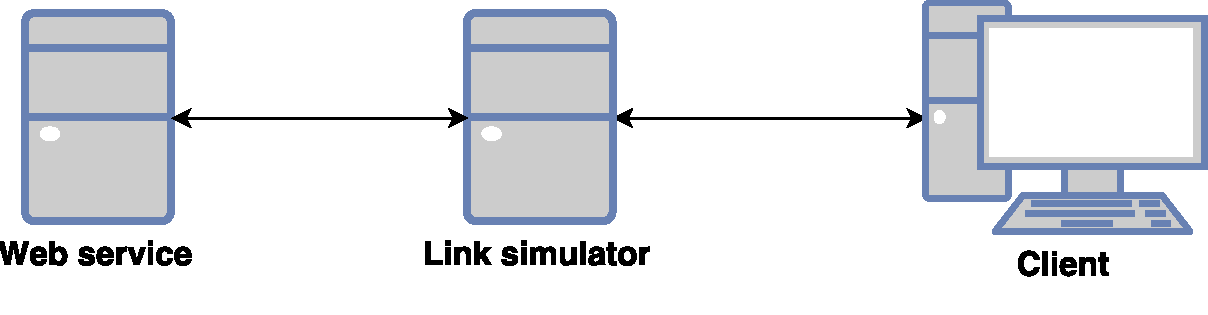
\includegraphics[scale=0.6]{images/testing_environment.pdf}
\caption{Testing environment}
\label{figure-testing-environment}
\end{figure}

The server and client are assigned an IP address in two different subnets.
This is done by the Linux network interface administration program
\textit{ifconfig}. In \cref{listing-ifconfig-client} the client machine is is
assigned the IP address 192.168.2.44.

\begin{lstlisting}[frame=single, caption="Configuring a network interface of the router", label=listing-ifconfig-client]
ifconfig eth0 192.168.2.1 up
\end{lstlisting}

After setting up the IP addresses we need to configure the routing so that the
kernel know where to route the network traffic. In this case we want all
traffic to go through the routing machine. In \cref{listing-routing} we
configure all IP traffic bound for the subnet 192.168.1.X to be routed through
the router machine with IP 192.168.2.1.

\begin{lstlisting}[frame=single, caption="Configuring routing rules for the client", label=listing-routing]
ip route add unicast 192.168.1.0/24 via 192.168.2.1
\end{lstlisting}

\subsubsection{Emulating different types of networks}

Since all network traffic passes through the routing machine, we can control
the flow of IP packets here. As previously discussed, we use NetEm.  For each
network configuration, a bash script is run. This script configures the
network interfaces in order to get the correct network behaviour. Both
interfaces are configured so the network is symmetrical in both directions.

\subsection{Tactical Broadband Setup}

Although testing on regular machines with emulated network gives us a good
indication, to validate the results we also performed tests on military
communication equipment. The setup is illustrated in
\cref{figure-radio-testing-environment}. It is point-to-point setup with two
radios, without any multi hop functionality. The radios have capacity to work as
a multi hop \gls{manet}, but this was not tested in this thesis.

\begin{figure}[h]
\centering
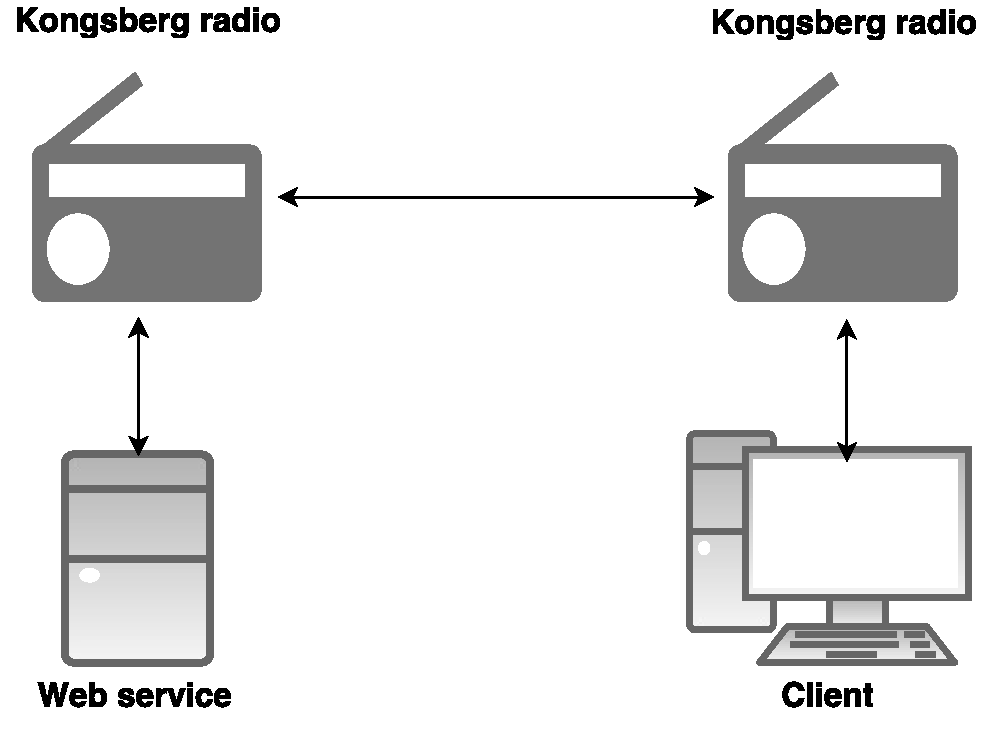
\includegraphics[scale=0.6]{images/radio_testing_environment.pdf}
\caption{Testing environment}
\label{figure-radio-testing-environment}
\end{figure}

\subsection{Proxy setup}

In order to enable the applications to tunnel all their HTTP traffic through our
proxy, we needed a way to setup a proxy without altering the applications
themselves. Fortunately, Java provide mechanisms to deal with
proxies\cite{oracle-proxy}. We configured the \gls{jvm} to get the applications
to tunnel all HTTP traffic through our proxy. This is done by setting properties
to the \gls{jvm}:


\begin{lstlisting}[frame=single, caption="Setting a proxy on the \gls{jvm}", label=test]
java -Dhttp.proxyHost=localhost \
-Dhttp.proxyPort=3001 \
-Dhttp.nonProxyHosts= \
-jar target/client.jar
\end{lstlisting}

In \cref{test} the application \textbf{client.jar} is started and all HTTP
traffic will go through the proxy server at localhost on port 3001.

\section{Test Execution}

For our tests we use originally used two different sets of applications. One for
W3C Web services and one for RESTful  Web services. While W3C web Services only
uses HTTP simply as a transport mechanism, REST utilizes the different HTTP
methods to indicate which operation to perform on a resource. Each test scenario
was therefor performed with both a W3C Web service application and RESTful Web
service application. Each service is deployed in Glassfish 4, while the client
is executed either from the command line or directly from the Netbeans IDEA.
Data being sent between the client and server is by default sent uncompressed.

During testing we discovered that especially CoAP was very sensitive to the
size of the messages being sent. We therefor developed a test application that
allowed the client to request a number of bytes from the server. This allowed us
to see how CoAP performed with different message sizes.

\subsection{NFFI W3C Web service}

For the purpose of testing W3C Web service applications we created a mock system
which allows a client to request a service to report positions of friendly
forces. The position reports use the \gls{nffi} format, which has an associated
XML schema with it. One test run is illustrated in \cref{figure-nffi-flow} and
consist of the client making a HTTP POST request to the Web service. Associated
with the request is an XML payload which tells the Web service which operation
to invoke. In our case, the service then returns an XML message containing a
large number of positions in the NFFI format.

\begin{figure}[h]
\centering
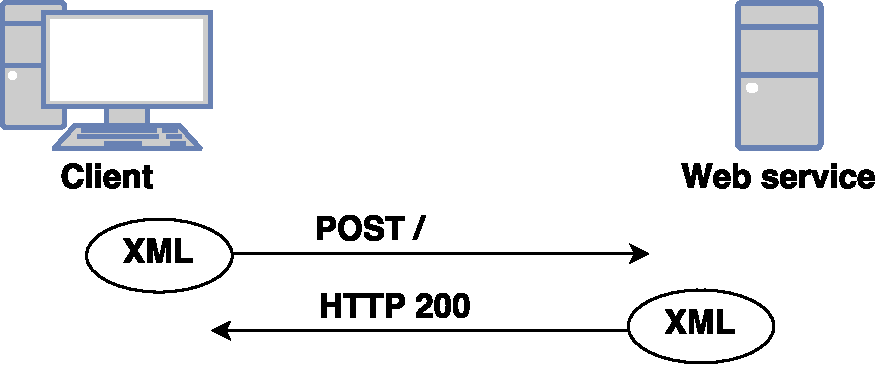
\includegraphics[scale=0.6]{images/nffi_flow.pdf}
\caption{NFFI Web service}
\label{figure-nffi-flow}
\end{figure}


\subsection{RESTful car Web service}

The RESTful Web service is an example service keeping order of cars in a ``car
system''. The service exposes an \gls{api} which offers different operations to
manage the car system. Clients can invoke these operations by using HTTP
requests and utilizing the associated HTTP method to indicate what to do with an
resource. Since RESTful services are payload agnostic, we choose JSON to
represent the data being sent between the server and the client. JSON is a
lightweight data-format. Each test run consist of a client sequentially invoking
the server with different API requests. The most common HTTP-methods GET, PUT,
POST, and DELETE are all part of the testing. An example, not inclusive, test run
is illustrated in \cref{figure-rest-flow}.

\begin{figure}[h]
\centering
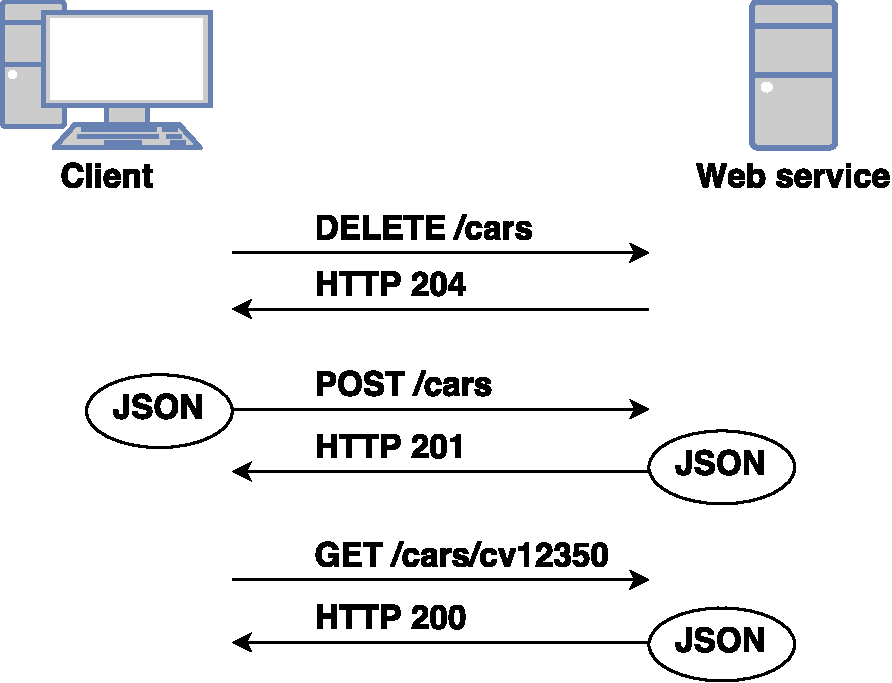
\includegraphics[scale=0.6]{images/rest_flow.pdf}
\caption{RESTful car service}
\label{figure-rest-flow}
\end{figure}


\subsection{Request size application}

This application allowed us to test with different message sizes.

\subsection{Test parameters}

The tests was performed with the following parameters.

\begin{itemize}
	\item GZIP compression on/off.
	\item Without and with proxies.
    \item Transport protocol used.
\end{itemize}


\section{Function tests}

The first phase of the testing was performed without any actual intended
limitations to the network. The objective of this testing is to validate that
the proxy is working correctly and have a benchmark to compare other results
with. This phase was again divided into two phases, one without the usage of
proxy and one with. Doing this allowed us to investigate any potential
overhead associated with the usage of the proxy. We used the NetEm setup with
a third machine acting as a router, although without any NetEm limitations
turned on.


\subsection{Results and Analysis}

Enabling compression yields an improvement in the performance, especially for
W3C Web services which had much larger messages. We also notice that HTTP and
CoAP has a almost identical performance, while AMQP has significant longer
average response time. Furthermore we can observe that the default solution
without proxies has the best performance in this unlimited network.

\begin{figure}[H]
\center
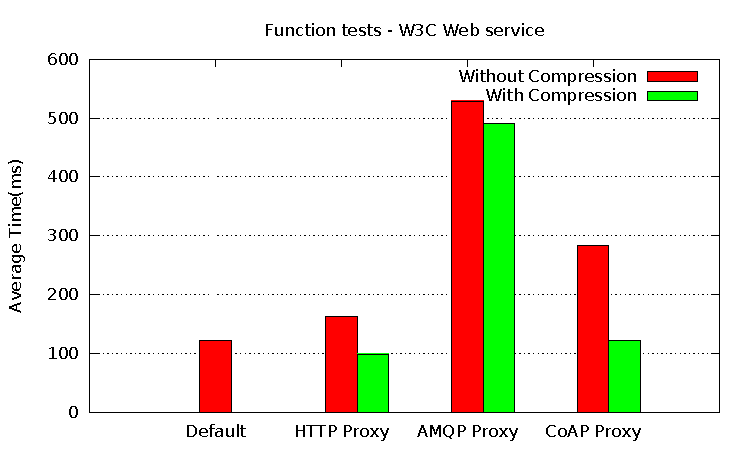
\includegraphics[scale=0.75]{../results/function_tests/nffi/out.pdf}
\caption{NFFI Web service results}
\end{figure}

\begin{figure}[H]
\center
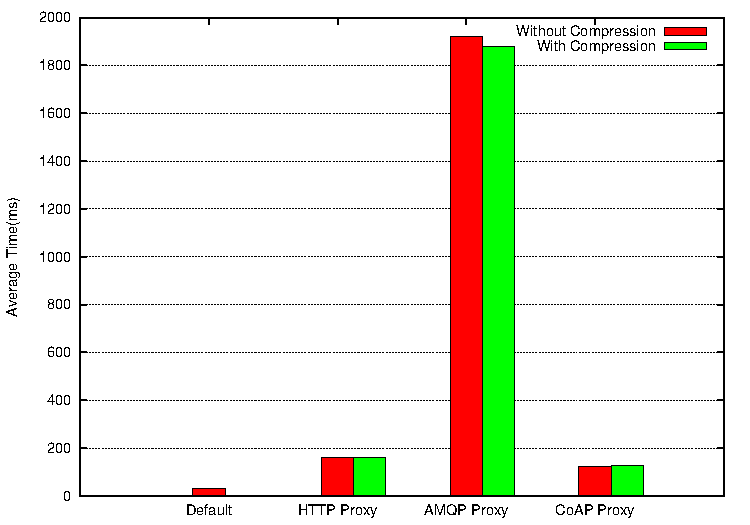
\includegraphics[scale=0.75]{../results/function_tests/rest/result.pdf}
\caption{REST results}
\end{figure}


\section{DIL Tests - Disconnected}

In this scenario we evaluate  the performance with the DIL characteristic
\textit{disconnected}, which refers to the network suddenly going down when the
application is sending data. The objective of this testing is to evaluate how
the proxy manages disconnects over longer periods of time. We define the success
criteria for this test to be that the client is able to eventually process his
request after the connection is reestablished. The client HTTP request should
not be interrupted in any way, other then it taking longer time to process the
request.

\subsection{Execution}

 The tests are performed on a unlimited network. During testing the Ethernet
 cable between the client machine and the router was removed for about 60
 seconds. It was then reconnected.

\subsection{Results and Analysis}

For both the REST and W3C Web service test scenarios the results were identical.
Without using proxies, the connection timed out and the applications were unable
to continue. With proxies the connection did not time out, and the protocols
retransmission mechanism were able to continue transmission when connection was
reestablished.

\begin{table}[h!]
\begin{tabular}{| l | l |}
\hline
  \textbf{Test} & \textbf{Result} \\ \hline
  Without proxy & Connection timeout \\ \hline
  Proxy with HTTP & Success \\ \hline
  Proxy with AMQP & Success \\ \hline
  Proxy with CoAP & Success \\ \hline
\end{tabular}
\caption{NFFI Web service results}
\end{table}

\begin{table}[h!]
\begin{tabular}{| l | l |}
\hline
  \textbf{Test} & \textbf{Result} \\ \hline
  Without proxy & Connection timeout \\ \hline
  Proxy with HTTP & Success \\ \hline
  Proxy with AMQP & Success \\ \hline
  Proxy with CoAP & Success \\ \hline
\end{tabular}
\caption{RESTful Web service results}
\end{table}



\section{DIL Tests - Intermittent}

\textit{Intermittent} refers to the network connection being lost, but then
regained again. The objective of this testing is to evaluate how the proxy
manages frequent temporary loss of connections. The success criteria is the same
as for disconnected, the client should not notice any disruption of service.

\subsection{Execution}

Not done yet. Similar to disconnect.

\subsection{Results}

\begin{table}[H]
\begin{tabular}{| l | l |}
\hline
  \textbf{Test} & \textbf{Result} \\ \hline
  Without proxy & X \\ \hline
  Proxy with HTTP & X \\ \hline
  Proxy with AMQP & X \\ \hline
  Proxy with CoAP & X \\ \hline
\end{tabular}
\caption{W3C Web service results}
\end{table}

\begin{table}[H]
\begin{tabular}{| l | l |}
\hline
  \textbf{Test} & \textbf{Result} \\ \hline
  Without proxy & X \\ \hline
  Proxy with HTTP & X \\ \hline
  Proxy with AMQP & X \\ \hline
  Proxy with CoAP & X \\ \hline
\end{tabular}
\caption{RESTful Web service results}
\end{table}

\section{DIL Tests - Limited}

The third DIL characteristic, \textit{limited}, refers to different ways a
network can be limited. This includes high delays, packet loss and low
bandwidth. In this section we present the testing performed for the different
types of networks identified in \cref{table-network-types}.



\subsection{Satellite communication}

In this test scenario we emulate \gls{satcom}. With satellite communication
all data is relayed through an communication satellite in orbit around
the earth. This type of communication is characterized by its low data rate
and high delay.

\subsubsection{Results and analysis}

AMQP has a very long response time for both test scenarios, while also CoAP
struggles with large uncompressed XML messages of the NFFI service. For both
with and without compression, we observe that employing HTTP proxies yields a
small improvement of performance, compared to the default. We can also notice
that for the RESTful service, CoAP has better performance than default, and
similar performance to HTTP proxies.

\begin{figure}[H]
\center
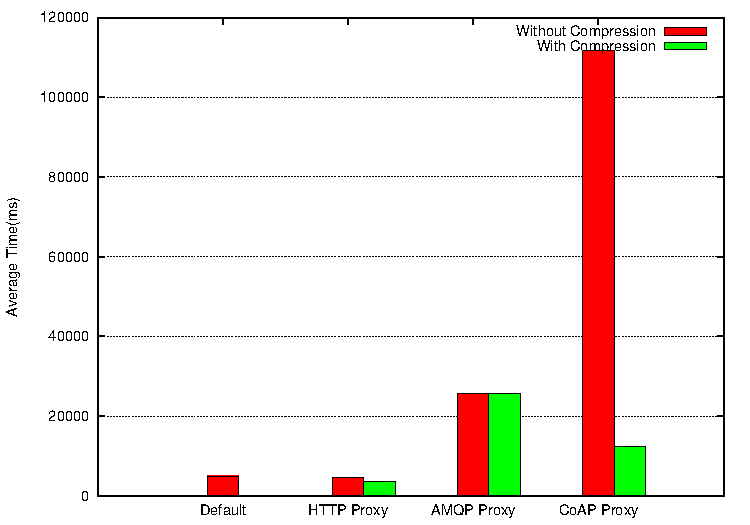
\includegraphics[scale=0.75]{../results/satellite/nffi/result.pdf}
\caption{NFFI Web service results}
\end{figure}

\begin{figure}[H]
\center
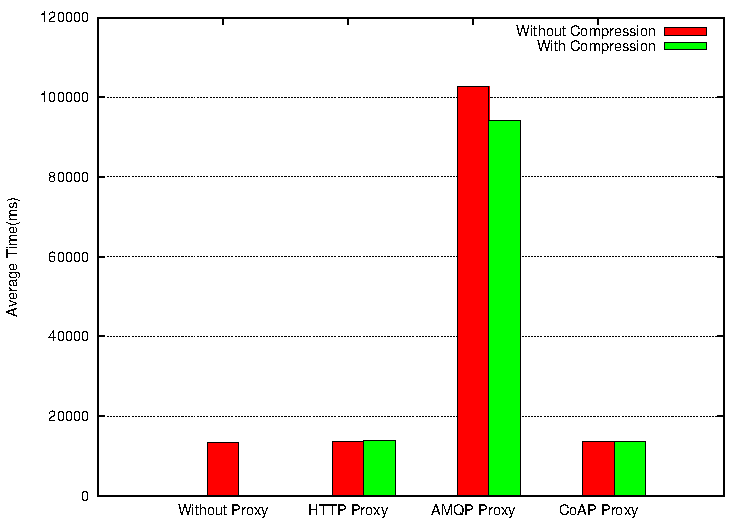
\includegraphics[scale=0.75]{../results/satellite/rest/result.pdf}
\caption{REST results}
\end{figure}

\subsection{Line-of-Sight}

In this test scenario we emulate so-called \gls{los} networks, which are
characterized by being a radio-based type of network with no physical obstacles
between the nodes in the network. High data rate, low delay and zero error.

\subsubsection{Results and analysis}

Again we notice CoAP really struggling with uncompressed XML messages, as well
as AMQP performing significantly poorer than the other protocols. However,
when the message is compressed CoAP has roughly equal performance as the
default. When we look on the RESTful test application results, we see that
CoAP performs better than default and HTTP with compressed messages.

\begin{figure}[H]
\center
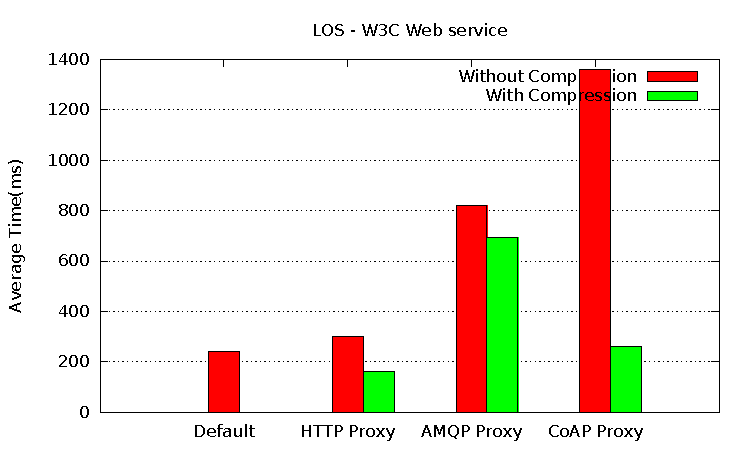
\includegraphics[scale=0.75]{../results/los/nffi/out.pdf}
\caption{NFFI Web service results}
\end{figure}

\begin{figure}[H]
\center
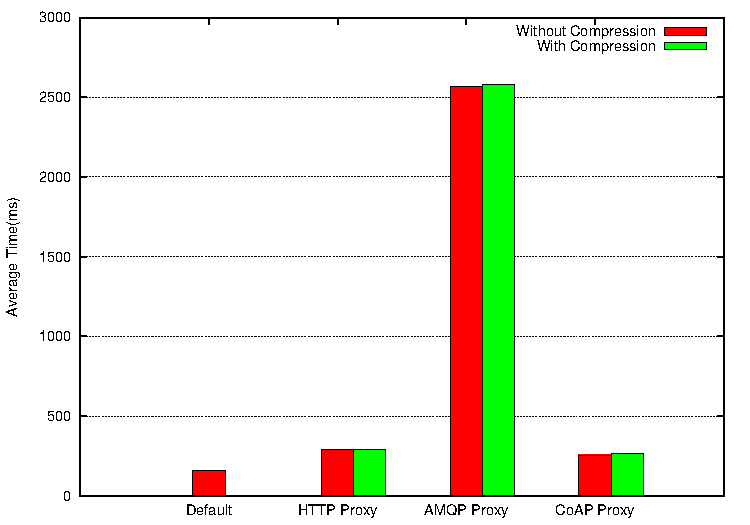
\includegraphics[scale=0.75]{../results/los/rest/result.pdf}
\caption{REST results}
\end{figure}



\subsection{WiFi 1}

With this type of network we emulate communication over WiFi where the
conditions are relatively good. The data rate is high, the delay is moderate
and the packet error rate is around 1 \%.

\subsubsection{Results and analysis}

HTTP proxies with compression enabled yields the best performance. CoAP has
worse performance than the HTTP proxies, but roughly equal for the compressed
REST tests.


\begin{figure}[H]
\center
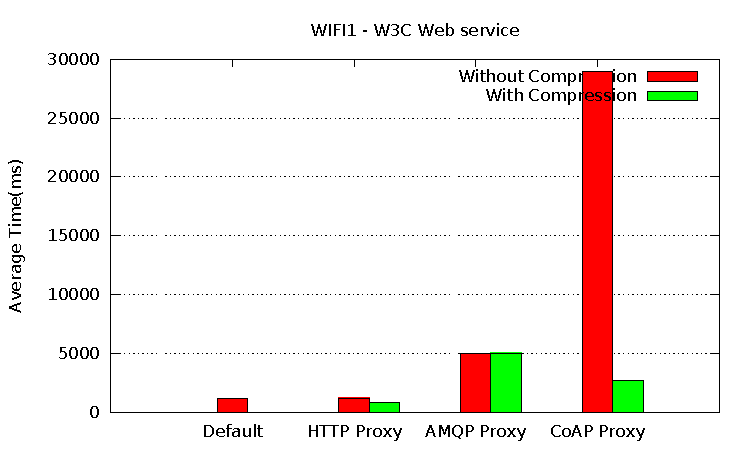
\includegraphics[scale=0.75]{../results/wifi1/nffi/out.pdf}
\caption{NFFI Web service results}
\end{figure}

\begin{figure}[H]
\center
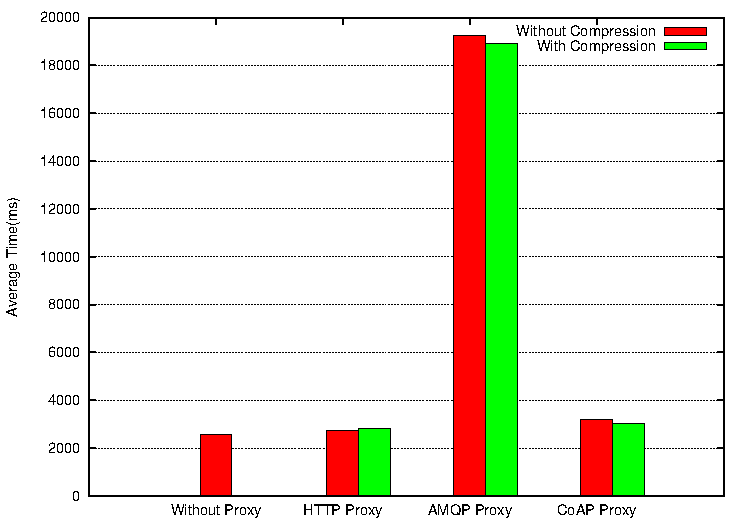
\includegraphics[scale=0.75]{../results/wifi1/rest/result.pdf}
\caption{REST results}
\end{figure}


\subsection{WiFi 2}

This type of network also emulate wireless communication, but instead in the
``outer'' areas of the wireless range. It has good data rate, moderate delay
and very high packet error rate(20 \%).


\subsubsection{Results and analysis}

Compared to WiFi 1, we see that all response times has increased
significantly. The importance of compression has increased, the tests with
compression turned on yields a large performance increase. In the uncompressed
NFFI test scenario, CoAP reached it's time out, and were unable to finish. In
the scenarios where CoAP did finish it still performed worse than default and
HTTP. HTTP proxies with compression yielded the best results.

\begin{figure}[H]
\center
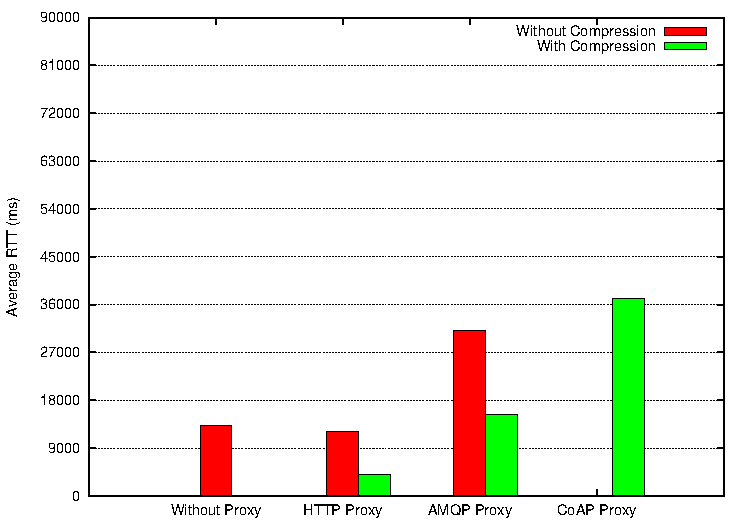
\includegraphics[scale=0.75]{../results/wifi2/nffi/result.pdf}
\caption{NFFI Web service results}
\end{figure}

\begin{figure}[H]
\center
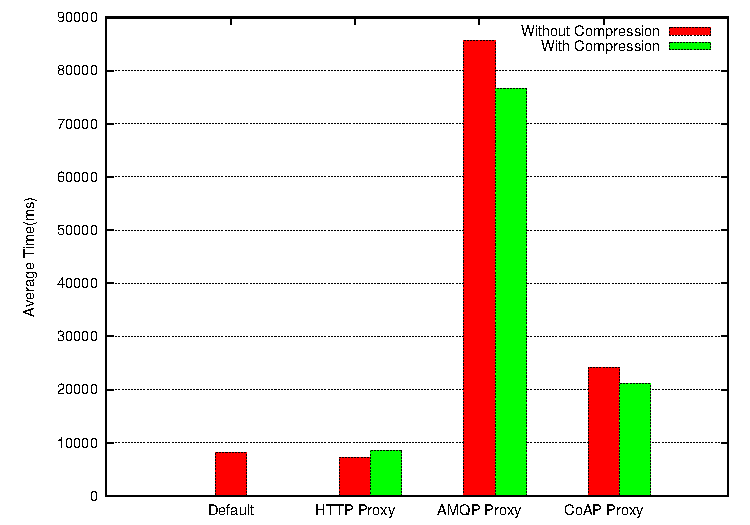
\includegraphics[scale=0.75]{../results/wifi2/rest/result.pdf}
\caption{REST results}
\end{figure}

\subsection{Combat Net Radio with Forward Error Correction}

\gls{cnr} is characterized by very low data rate, moderate timeout and packet
error rate on around 1 \%.


\subsubsection{Results and analysis}

Again we can observe the importance of compression in this type of networks.
CoAP has the best performance.

\begin{figure}[H]
\center
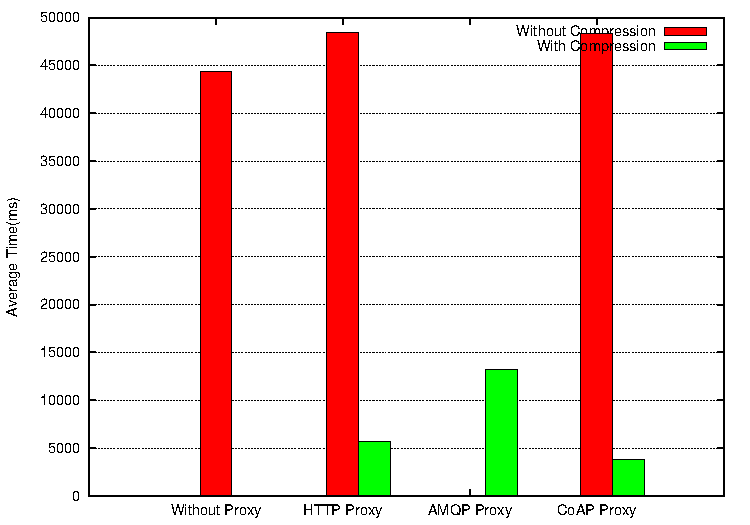
\includegraphics[scale=0.75]{../results/cnr/nffi/result.pdf}
\caption{NFFI Web service results}
\end{figure}

\begin{figure}[H]
\center
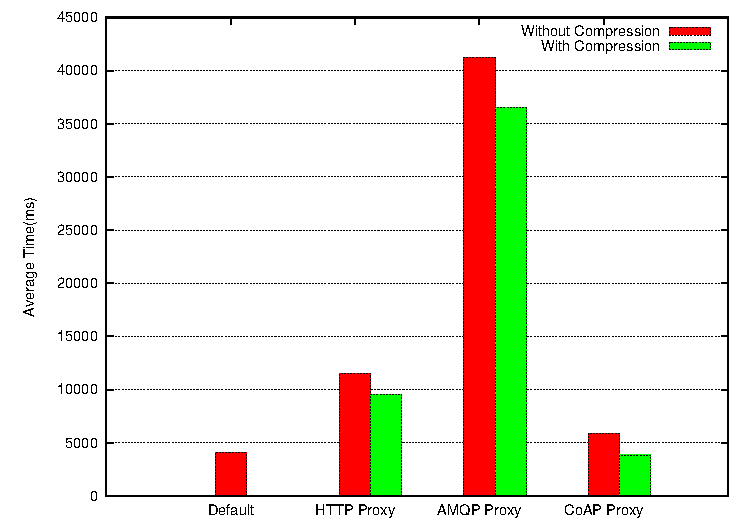
\includegraphics[scale=0.75]{../results/cnr/rest/result.pdf}
\caption{REST results}
\end{figure}

\begin{figure}[H]
\center
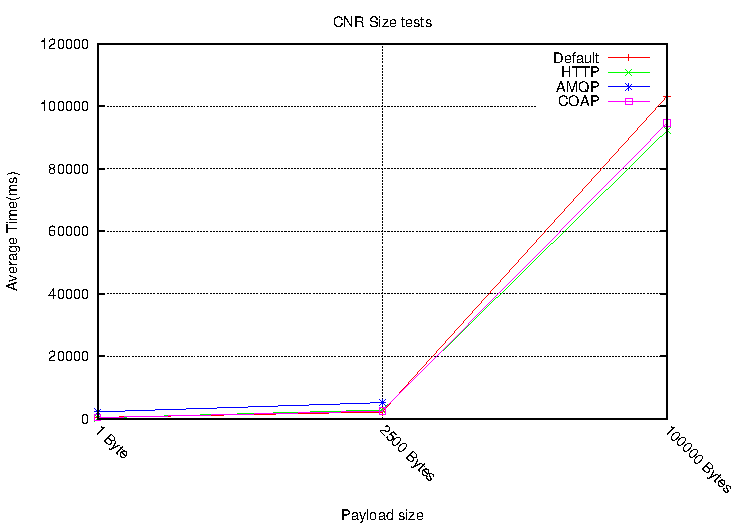
\includegraphics[scale=0.75]{../results/cnr/size/result.pdf}
\caption{Size request results}
\end{figure}


\subsection{EDGE}

About this type of network.

\subsubsection{Results and analysis}

\begin{figure}[H]
\center
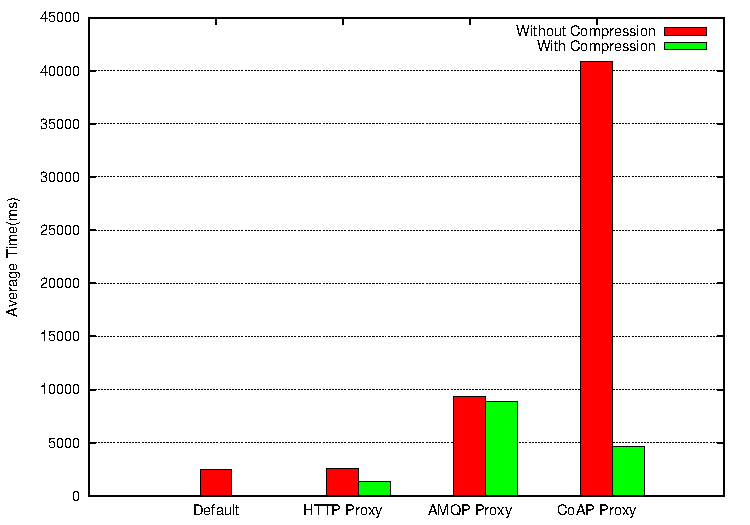
\includegraphics[scale=0.75]{../results/edge/nffi/result.pdf}
\caption{NFFI Web service results}
\end{figure}

\begin{figure}[H]
\center
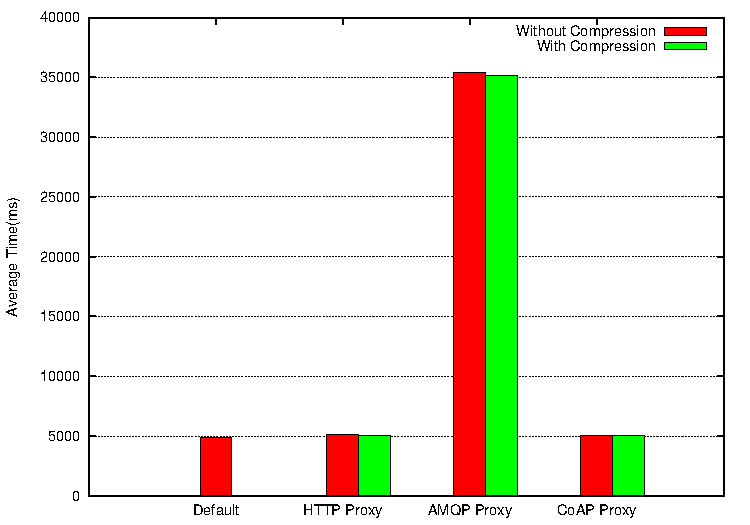
\includegraphics[scale=0.75]{../results/edge/rest/result.pdf}
\caption{REST results}
\end{figure}

\subsection{Kongsberg Radio}

Two KDA WM 600.


\subsubsection{Results and analysis}

For NFFI tests, compression yields a lot of increase in performance.

\begin{figure}[H]
\center
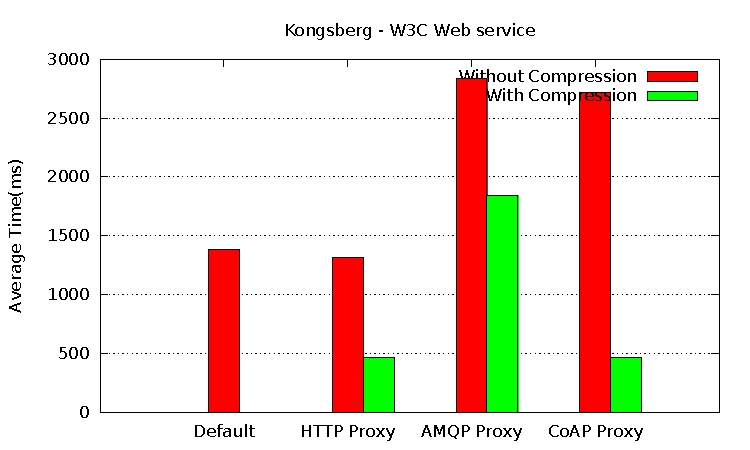
\includegraphics[scale=0.75]{../results/kongsberg/nffi/out.pdf}
\caption{NFFI Web service results}
\end{figure}

\begin{figure}[H]
\center
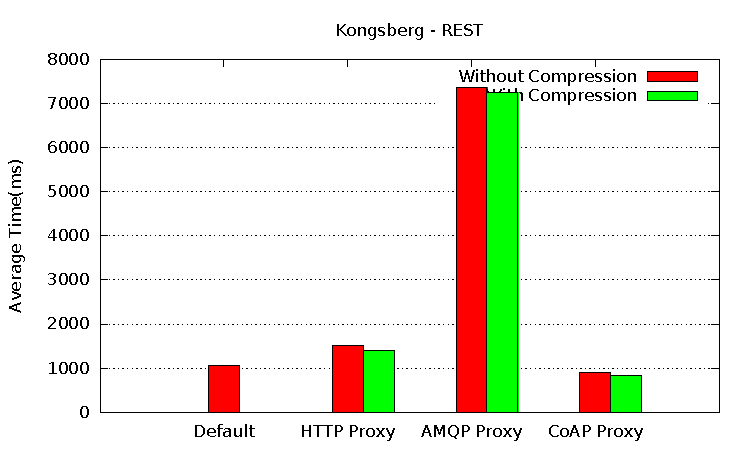
\includegraphics[scale=0.75]{../results/kongsberg/rest/out.pdf}
\caption{REST results}
\end{figure}



\section{Summary}

In this section the results from the tests are presented. These results lead up
to the discussion and conclusion in the next chapter.

\begin{itemize}
\item AMQP has the worst performance in almost every test scenario.
\item Compression almost always yields in performance increase.
\item CoAP struggles with larger messages.
\item CoAP has the best performance with smaller messages in networks with low data rate.
\end{itemize}

\begin{table}[h]
\begin{tabular}{| l | l | l |}
\hline
  \textbf{Network} & \textbf{NFFI Web service recommendation} & \textbf{REST service recommendation}\\ \hline
  \gls{satcom} & AMQP Proxy & 550 ms \\ \hline
  \gls{los} & X & X\\ \hline
  WiFi 1 & X & X \\ \hline
  WiFi 2 & X & X \\ \hline
  \gls{cnr} & X & X \\ \hline
  Edge & X & X\\ \hline
\end{tabular}
\caption{Recommendations}
\label{table-evaluation-summary}
\end{table}
